\documentclass[../main.tex]{subfiles}
\graphicspath{{\subfix{../figures/}}}
%
\title{用鱼骨图思考和分析问题}
%
\begin{document}
\maketitle
%
\section{鱼骨分析法}
鱼骨分析法又名因果分析法,由日本管理大师石川馨先生发展而来,
是一种透过现象看本质的分析方法,可以帮助我们快速找出引发问题的根本原因。

鱼骨分析法的基本原理是针对一个问题(作为鱼头),
列明产生问题的大要因(鱼骨主干),从大要因继续深入细分,
挖掘小要因(鱼骨分支),如此一层层挖掘分析下去,
直至找出可以解决问题的方法或者行动的步骤。
%
\begin{figure}[H]
  \begin{center}
    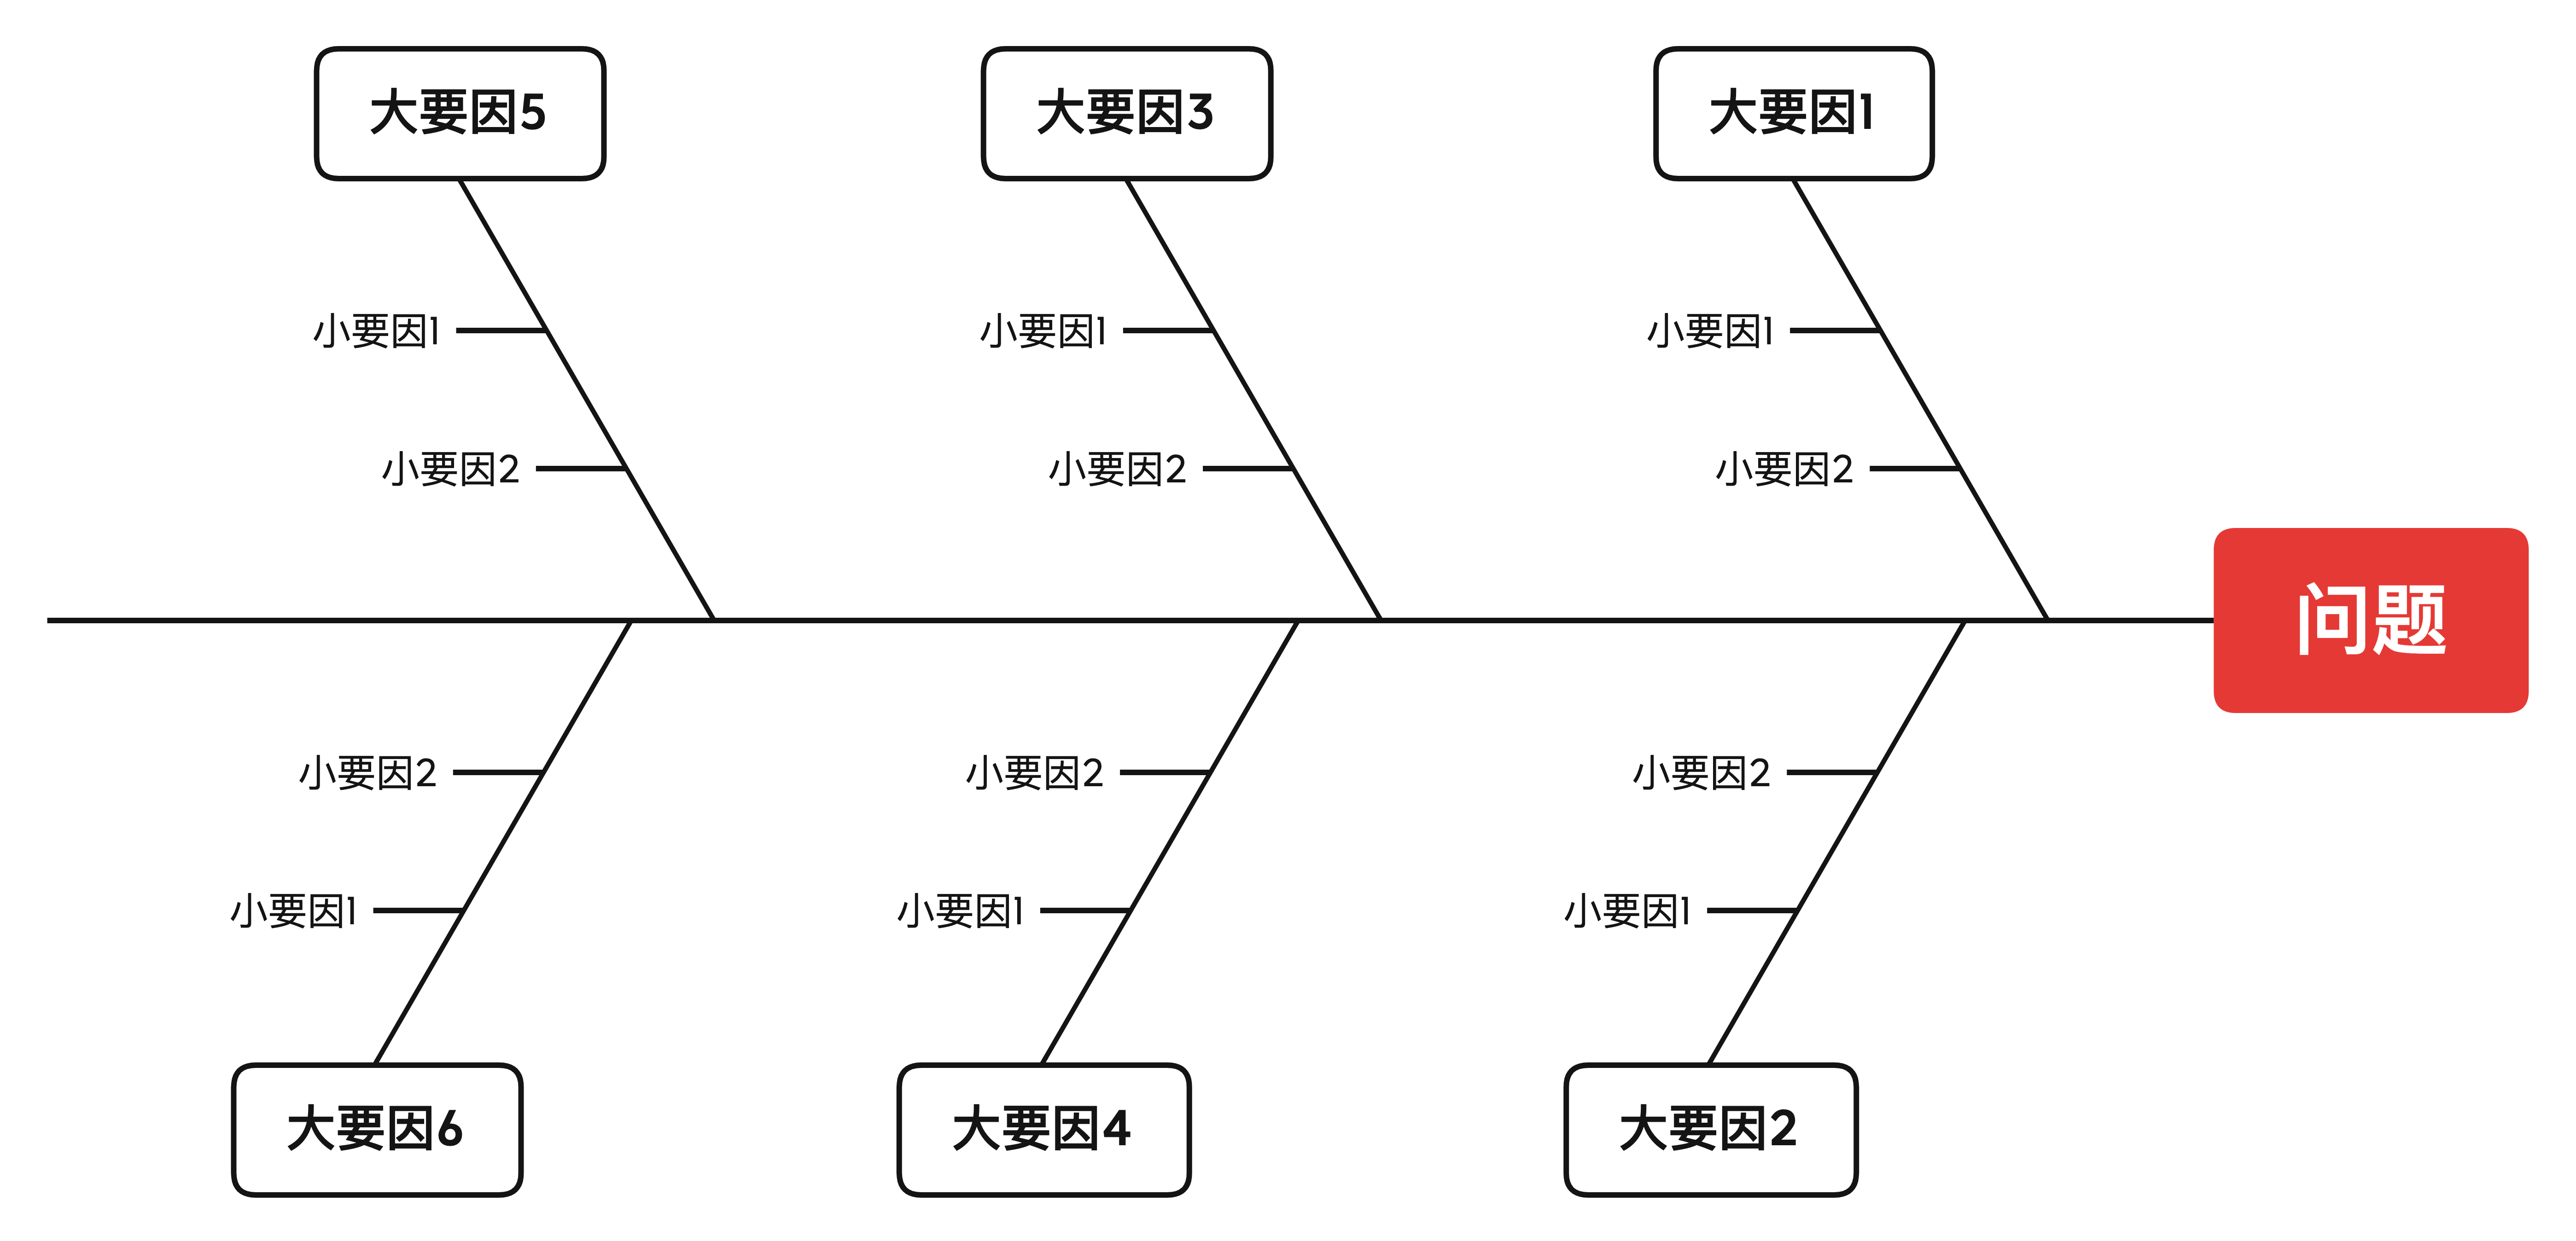
\includegraphics[width=0.50\textwidth]{鱼骨分析法_问题_要因.png}
  \end{center}
\end{figure}
%
常用的鱼骨图有原因型鱼骨图(鱼头在右)和对策型鱼骨图(鱼头在左)两种,
用来分析问题和解决问题。
下图即是一张分析营销推广效果不佳原因的鱼骨分析图,
分别从人员、过程、环境、渠道、内容、管理六大方面来分析本次推广效果不佳的原因。
%
\begin{figure}[H]
  \begin{center}
    \includegraphics[width=0.50\textwidth]{鱼骨分析法_营销推广效果不佳.png}
  \end{center}
\end{figure}
一张专业的鱼骨图,有利于让我们把注意力和精力集中到问题的本质上,
更深入地去思考和挖掘原因,从而更高效地找寻解决问题的方法。

接下来我们从具体的例子入手,和大家分享如何玩转鱼骨图结构。
%
\section{鱼骨图绘制步骤}
了解鱼骨分析法的基本原理后,可知鱼骨图的绘制过程并不复杂,
总的可以概括为以下四个步骤:
%
\begin{itemize}
  \item 明确要解决的问题,将问题写在鱼骨头。
  \item 从各个角度进行思考,找出各个要因,并在鱼骨主干上标出。
  \item 在要因上深挖,更深入地思考具体的细节,在鱼骨分支上标出。
  \item 仔细思考各个原因,找寻相应的解决思路。
\end{itemize}
%
以困扰当代年轻人的一大婚恋难题为例,
和大家一起来绘制一个简单的因果分析图。

首先,确定思考的问题。明确我们所面临的问题``为什么单身''后,
第一步即是打开 XMind 中的鱼骨图结构,把问题写在鱼头。
%
\begin{figure}[H]
  \begin{center}
    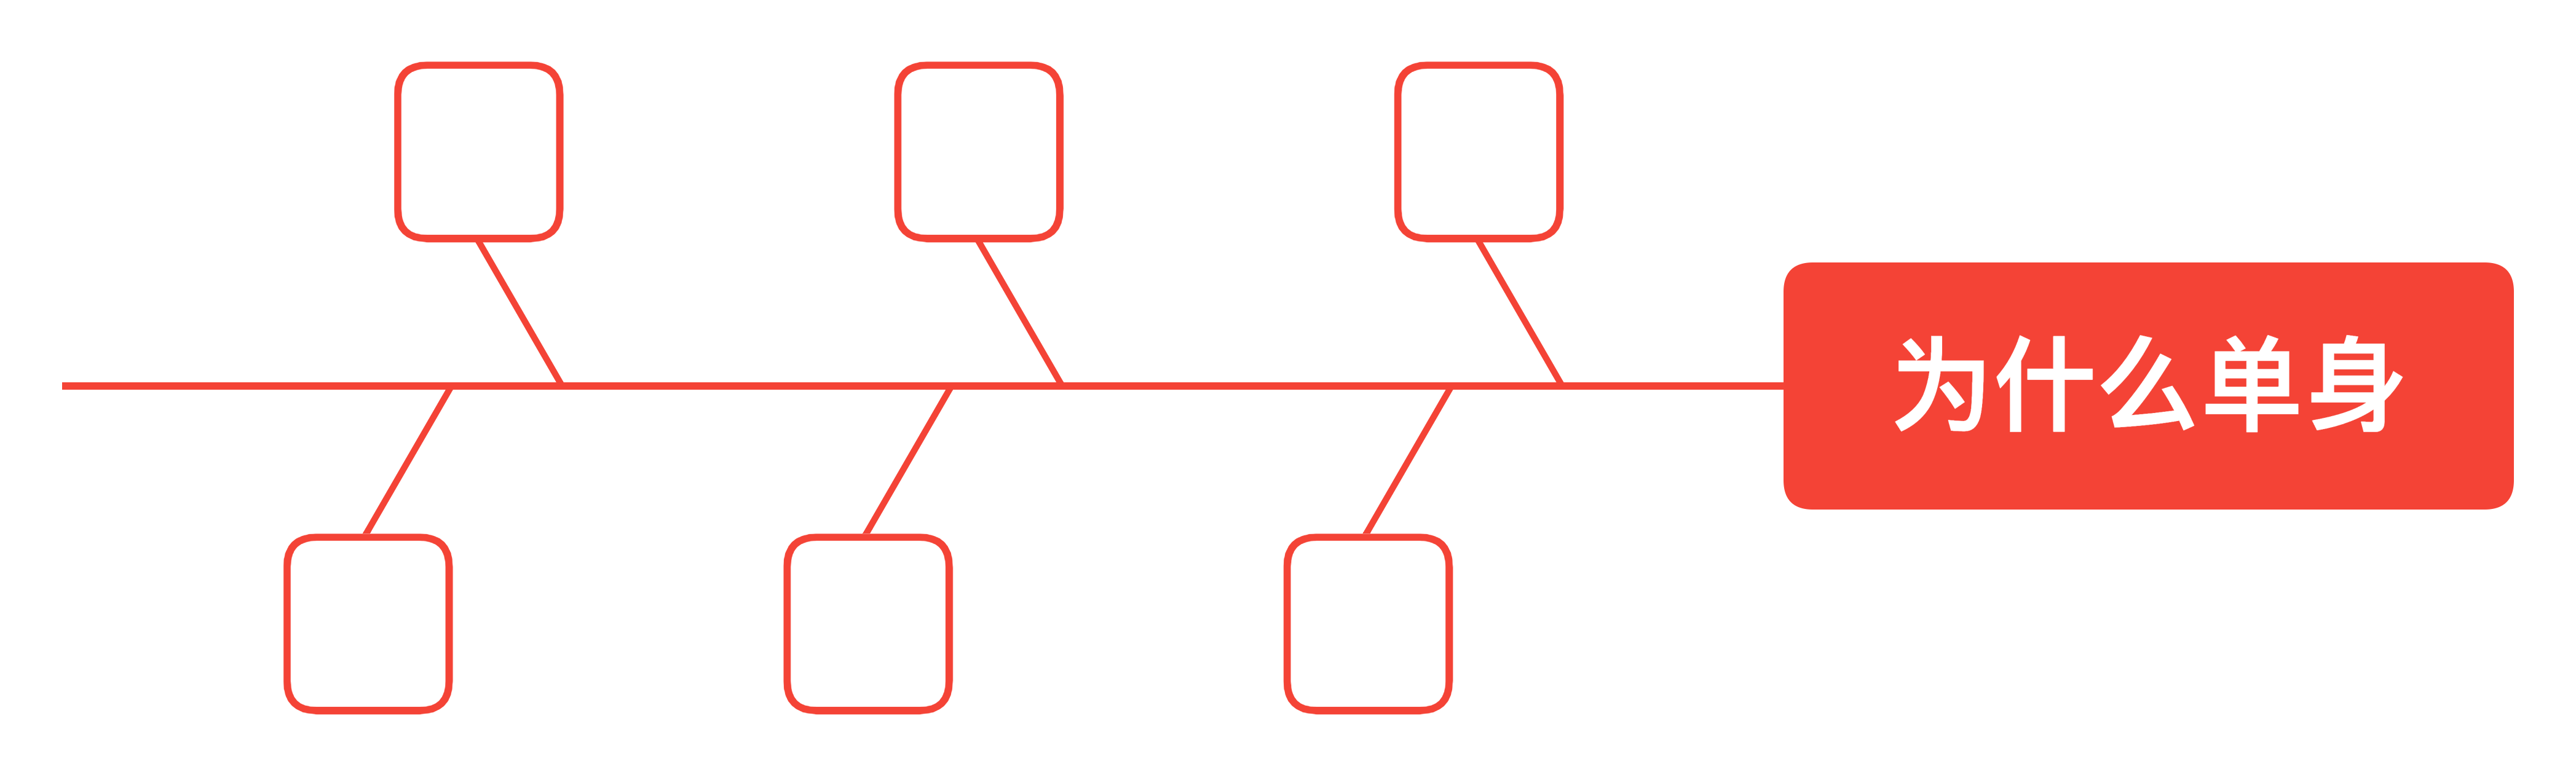
\includegraphics[width=0.50\textwidth]{鱼骨分析法_为什么单身.png}
  \end{center}
\end{figure}
%
接下来思考我们可以从哪些方面来思考和分解这个问题。
可能直接写出主因有点困难,可以用创建自由主题的方式在
XMind 的画布空白处罗列出各种我们可以想到的各种原因。
%
\begin{figure}[H]
  \begin{center}
    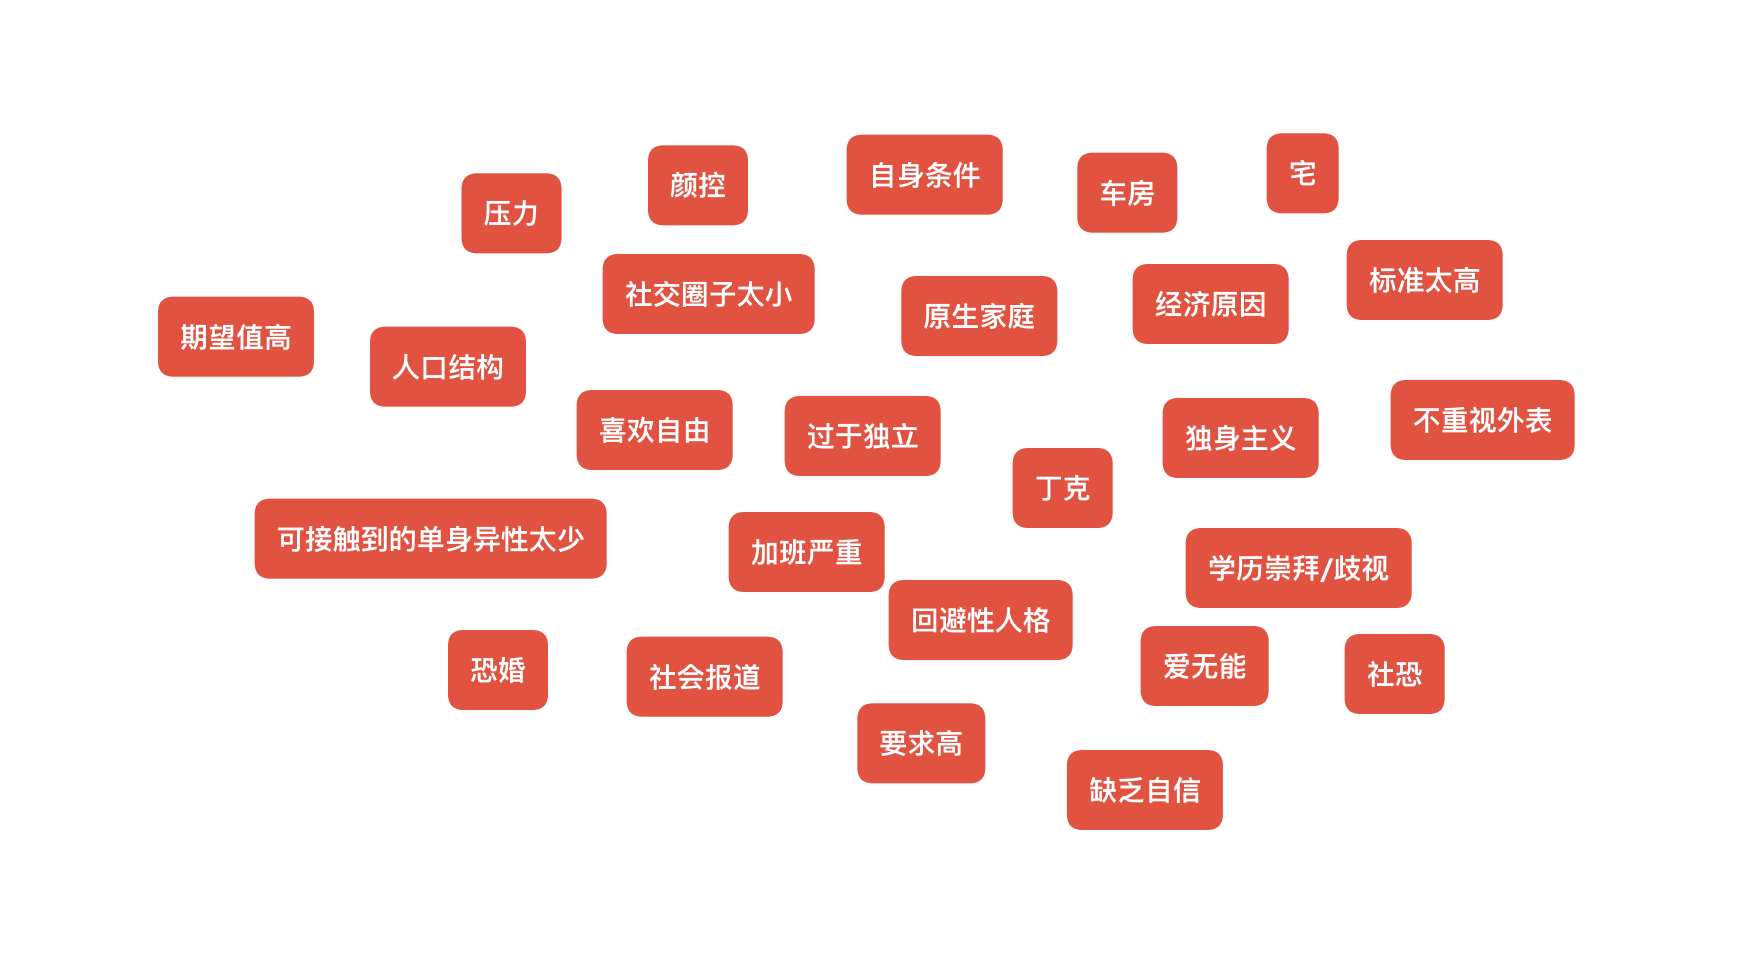
\includegraphics[width=0.50\textwidth]{鱼骨分析法_原因.png}
  \end{center}
\end{figure}
%
在这个基础上根据 MECE 原则(相互独立,完全穷尽)
进行思考维度的总结和抽象概括,并在鱼骨主干上标出,如下图。
%
\begin{figure}[H]
  \begin{center}
    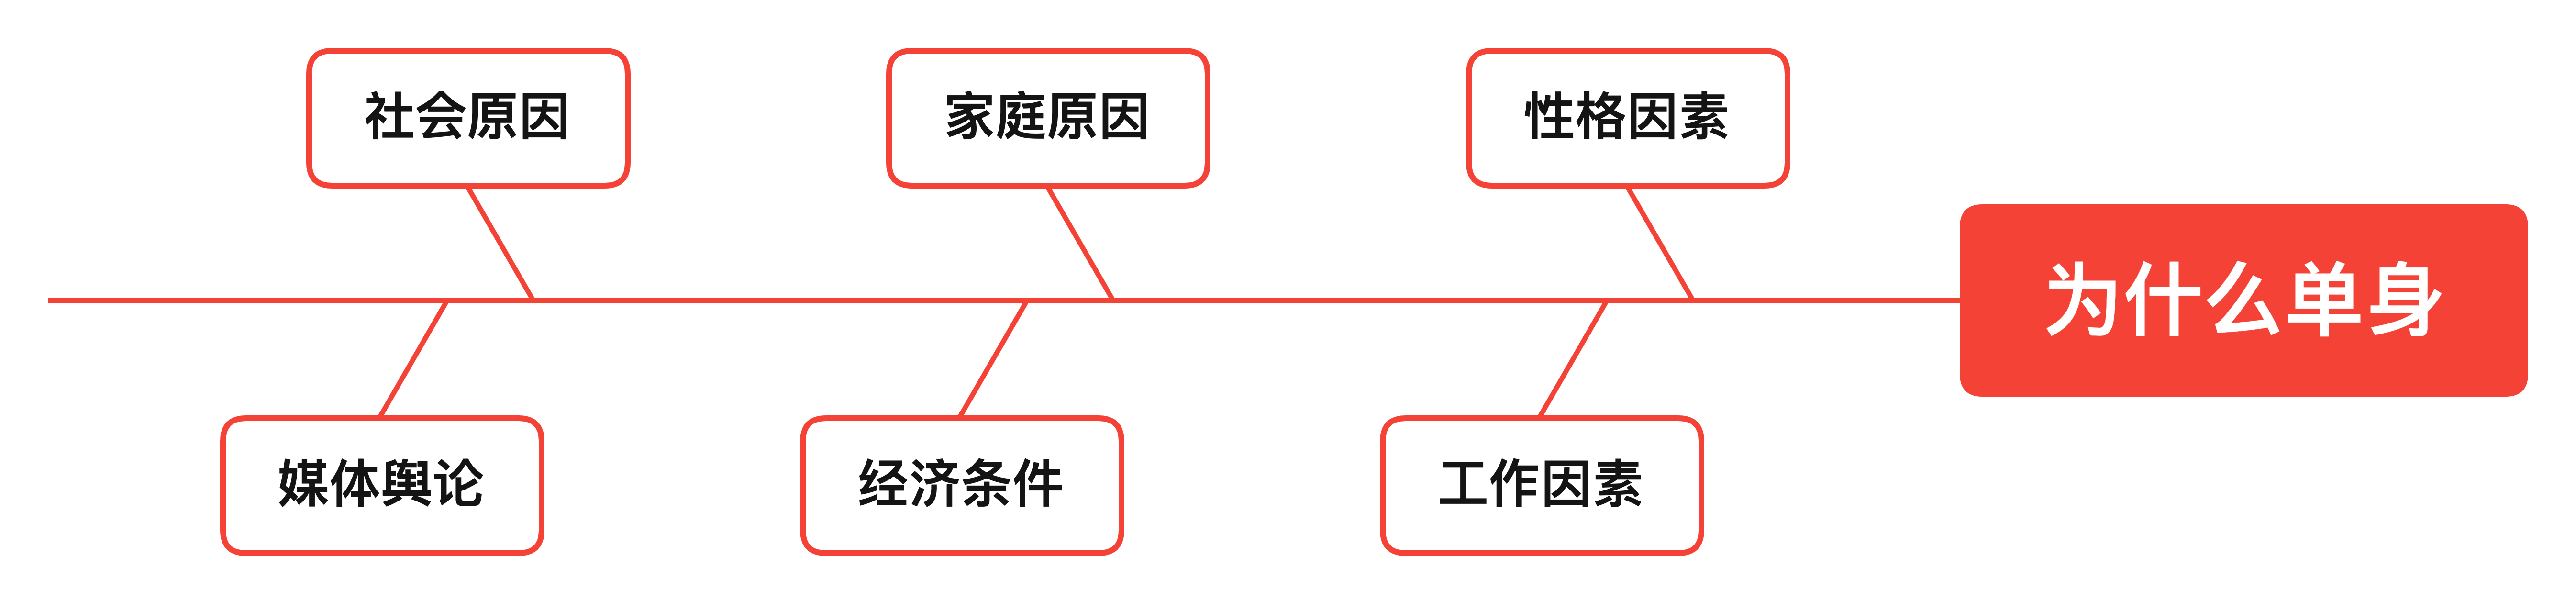
\includegraphics[width=0.50\textwidth]{鱼骨分析法_1.png}
  \end{center}
\end{figure}
%
然后将各个原因归类到各个维度中,并在此基础上进一步进行补充和发散。如下图所示。
%
\begin{figure}[H]
  \begin{center}
    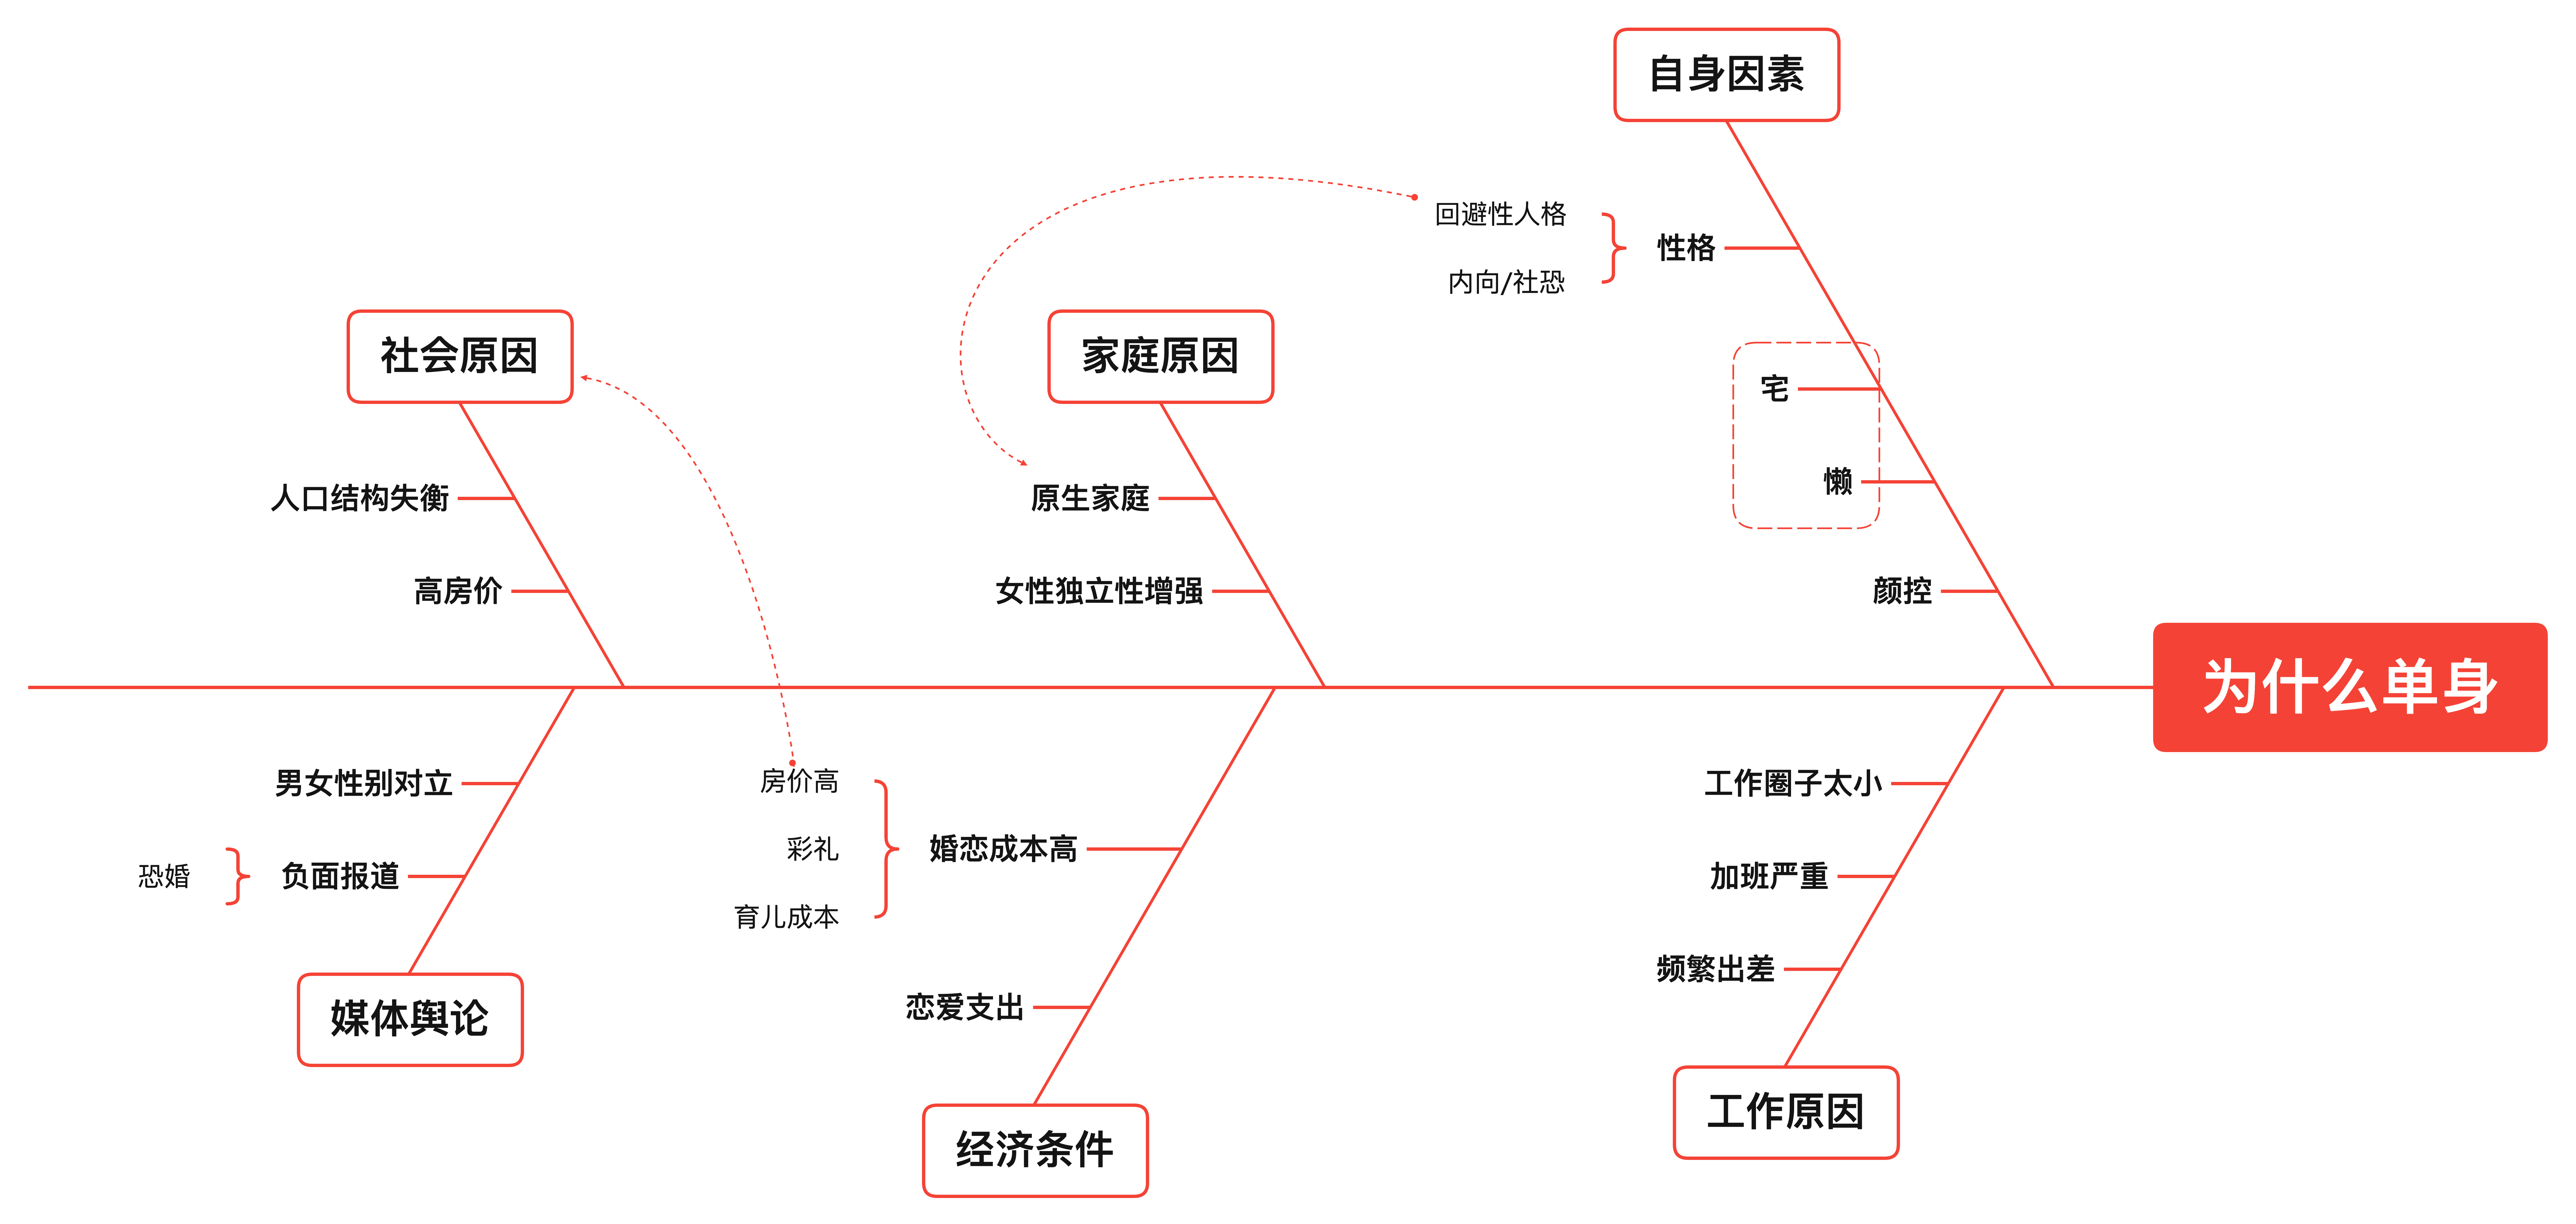
\includegraphics[width=0.50\textwidth]{鱼骨分析法_2.png}
  \end{center}
\end{figure}
%
当你思考将问题思考清楚后,可以从问题的原因入手,
思考相对应的解决方案,制作``如何脱单''的对策型的鱼骨图,如下图所示。
%
\begin{figure}[H]
  \begin{center}
    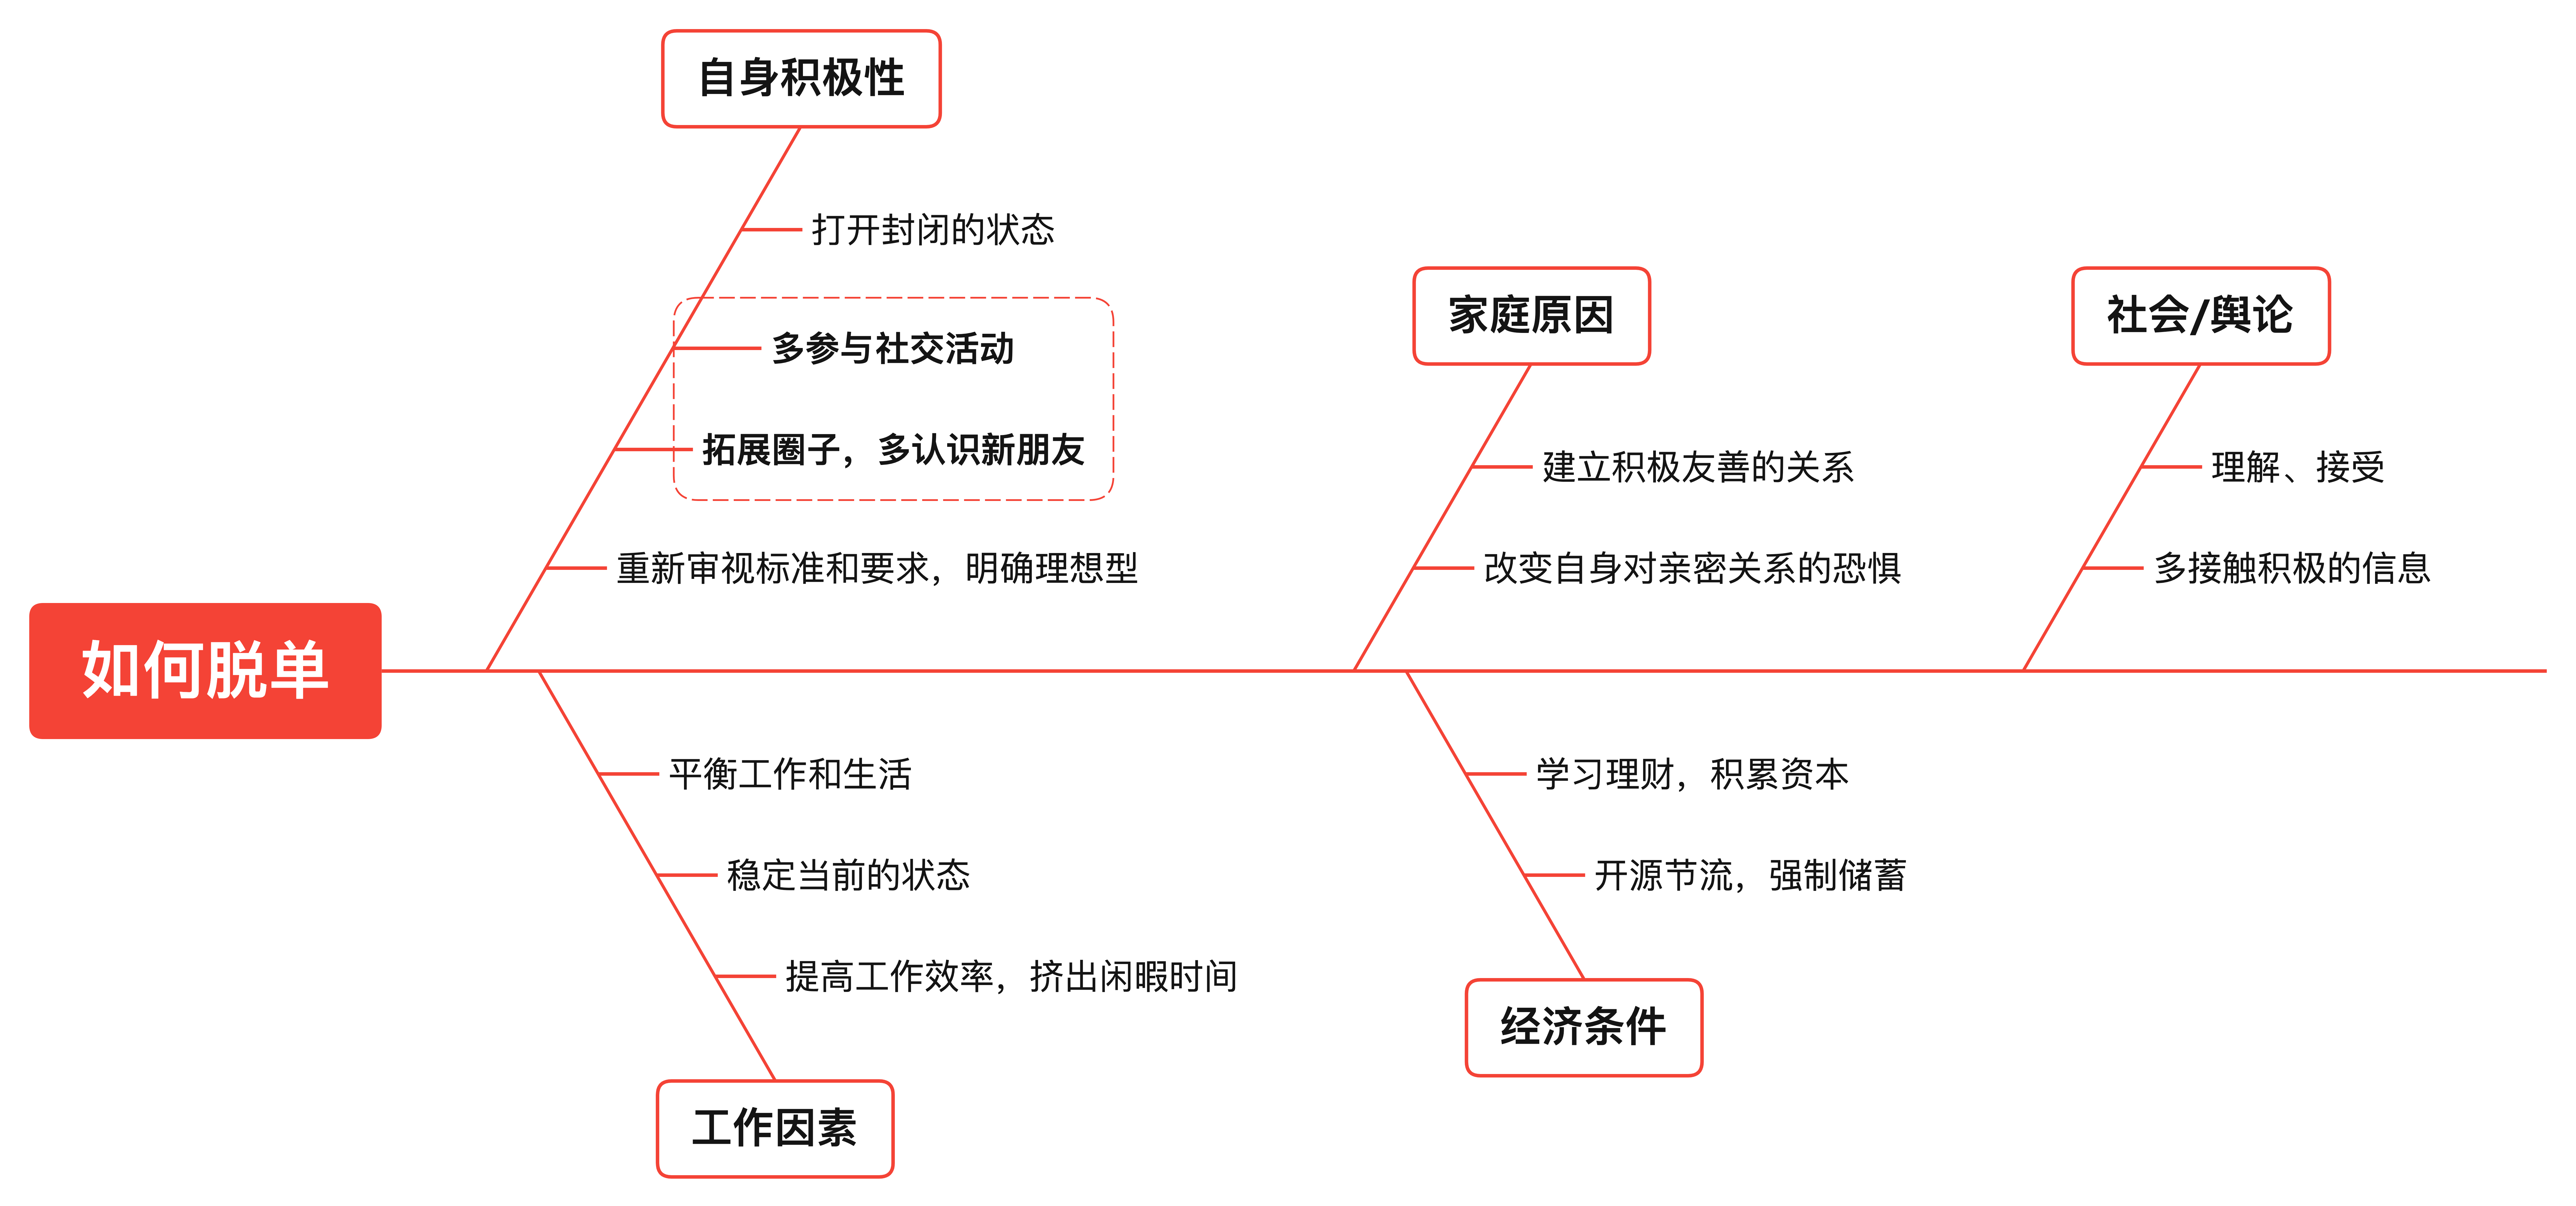
\includegraphics[width=0.50\textwidth]{鱼骨分析法_3.png}
  \end{center}
\end{figure}
%
当我们能思考清楚问题产生的本质时,找寻更好的解决方案才有可能。
想清楚如何做,有的放矢,执行效率才更高。
%
\section{鱼骨分析法的应用}
鱼骨分析法通过对问题的层层拆解,从表面的现象深挖问题的本质。
这种深入思考的框架可以应用在解决学习、工作、生活难题上,
可以用它来进行事件分析、因果分析、问题分析、对策分析等。

接下来举一些实际应用鱼骨分析法的例子。
%
\subsection{问题分析}
鱼骨分析法可应用于分析工作、生活中遇到的各种难题。
比如在思考营销计划是否周全时,可以试着建立一个诊断框架,
从``品牌是否存在问题-问题在哪里-为什么存在问题''的思考链路入手,
一步一步探寻造成问题的根本原因。
%
\begin{figure}[H]
  \begin{center}
    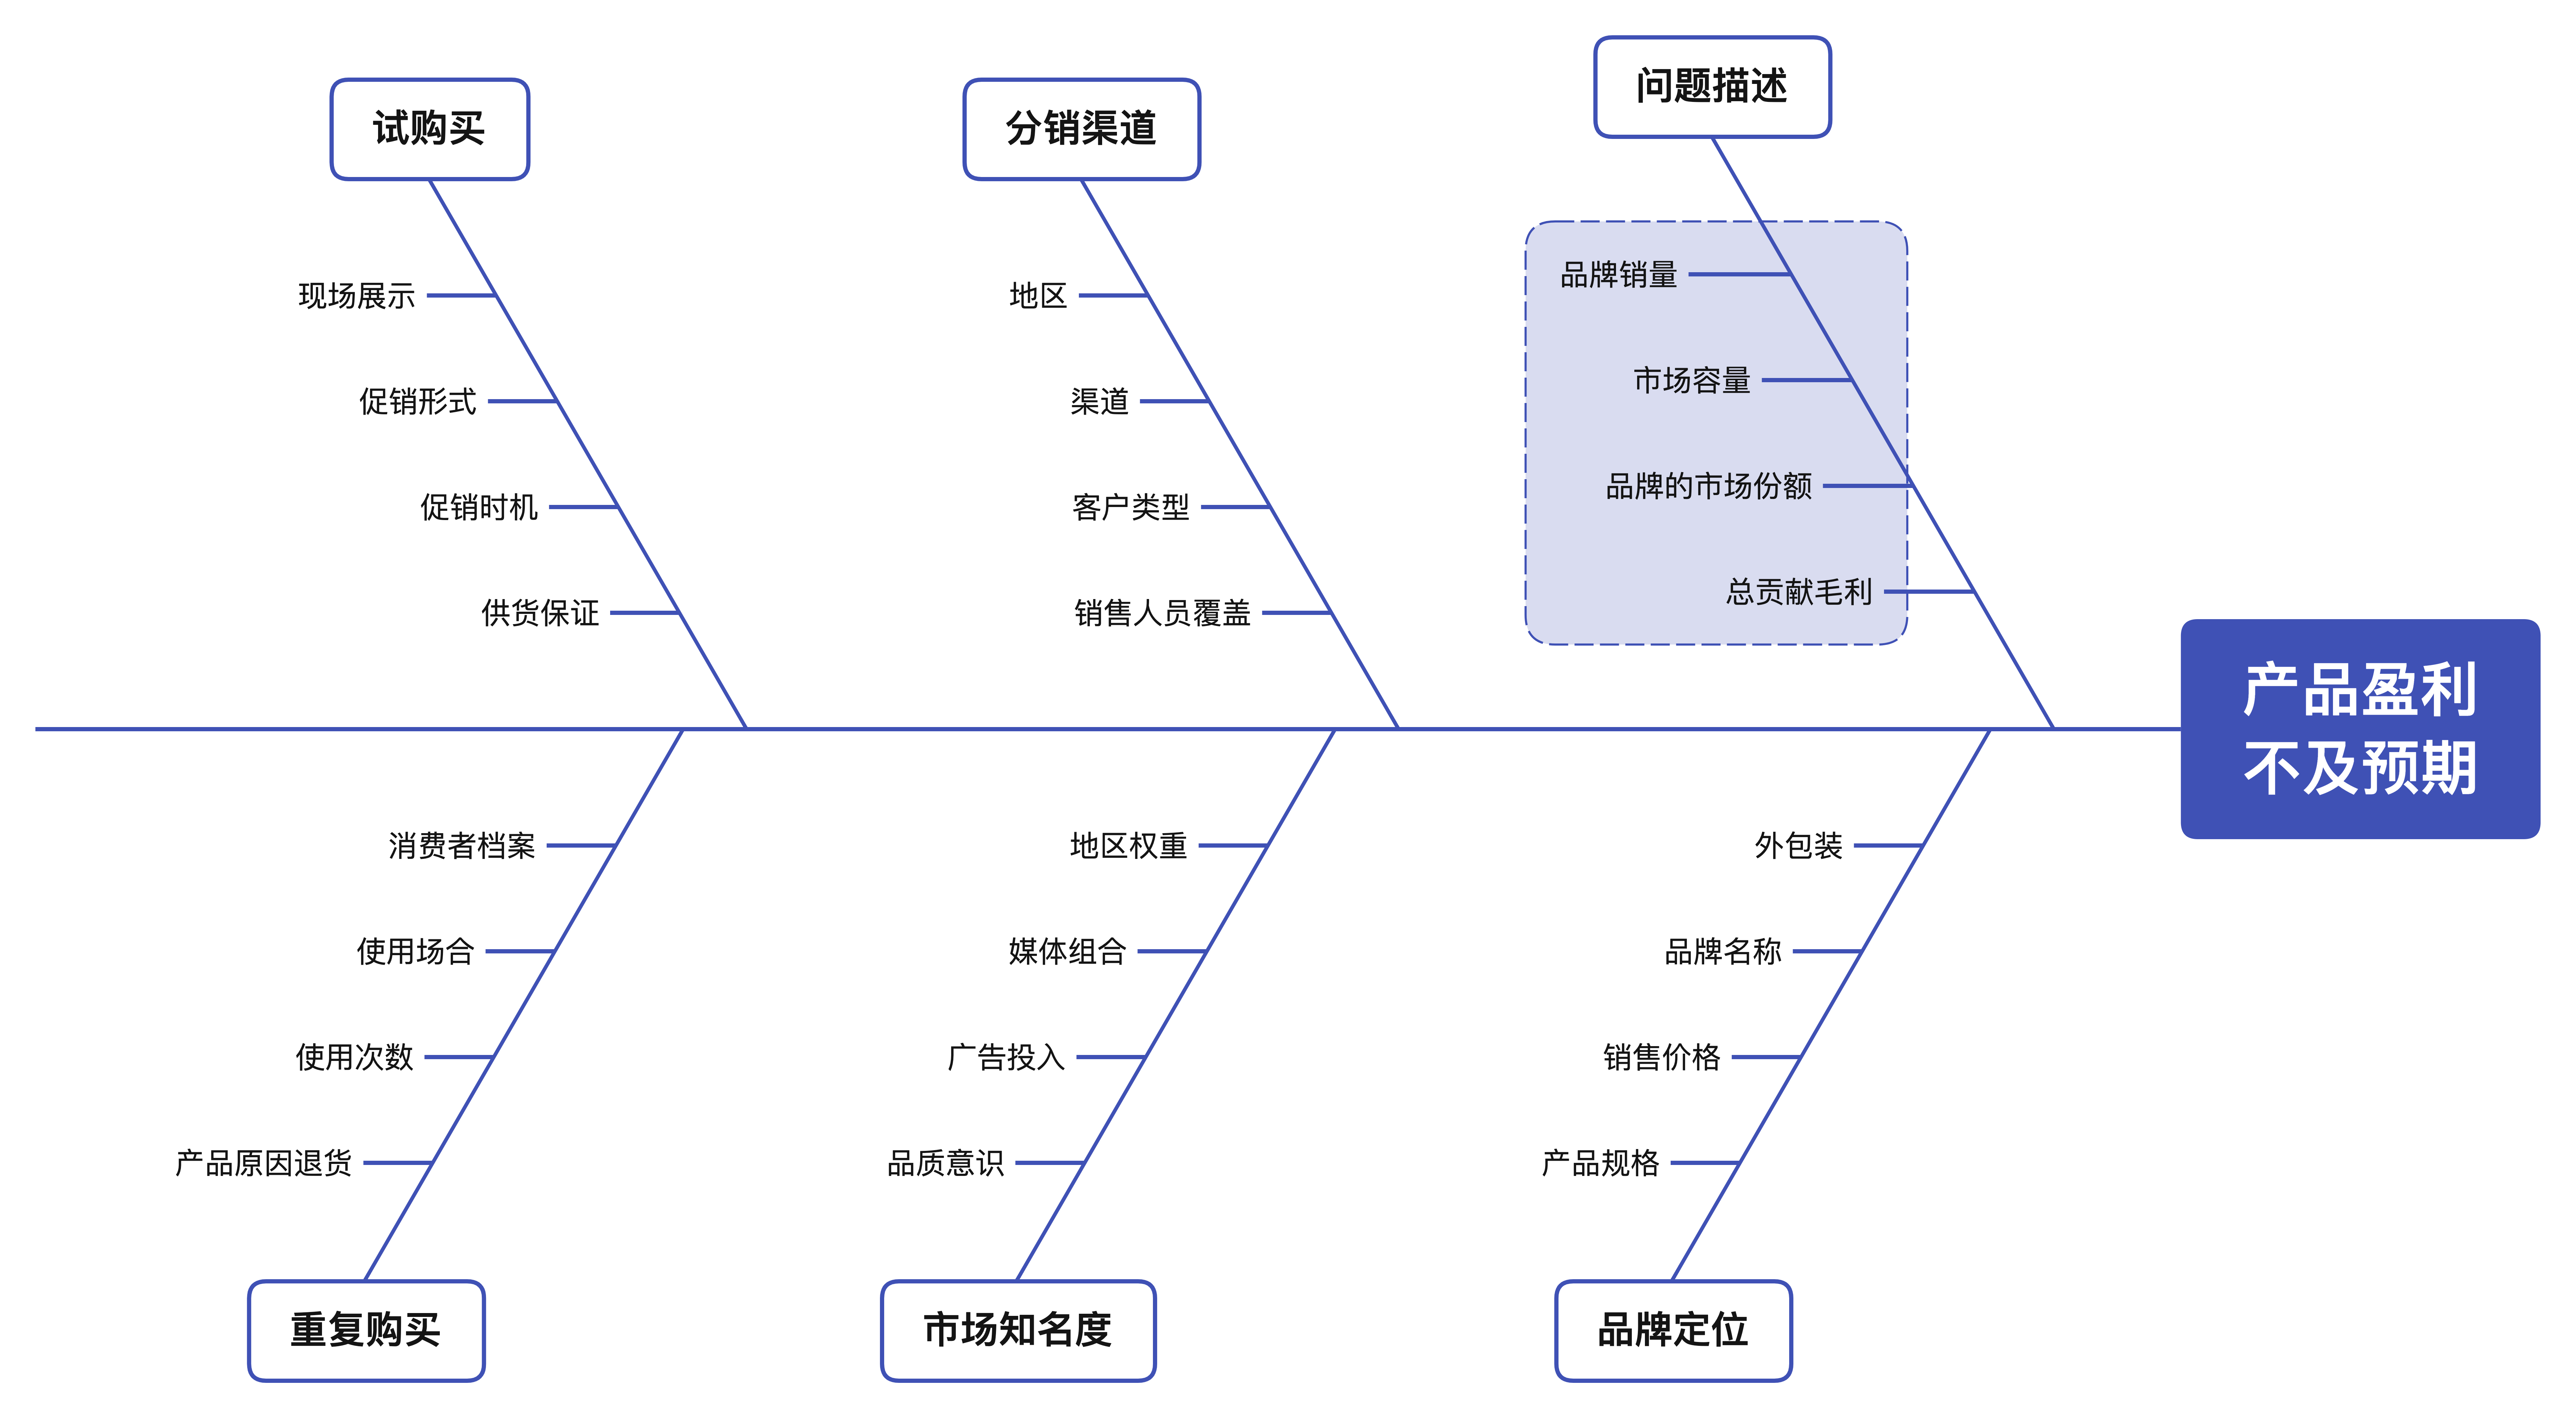
\includegraphics[width=0.50\textwidth]{鱼骨分析法_4.png}
  \end{center}
\end{figure}
%
鱼骨分析法让你建立思考问题的框架,尽可能全面地去分析问题可能产生的原因,
再根据现实情况一一验证,
找出问题的根本原因后制定相应的应对措施和改进方法。
比如企业在遇到招聘难题时可以用鱼骨分析法来分析自身存在的问题。
%
\begin{figure}[H]
  \begin{center}
    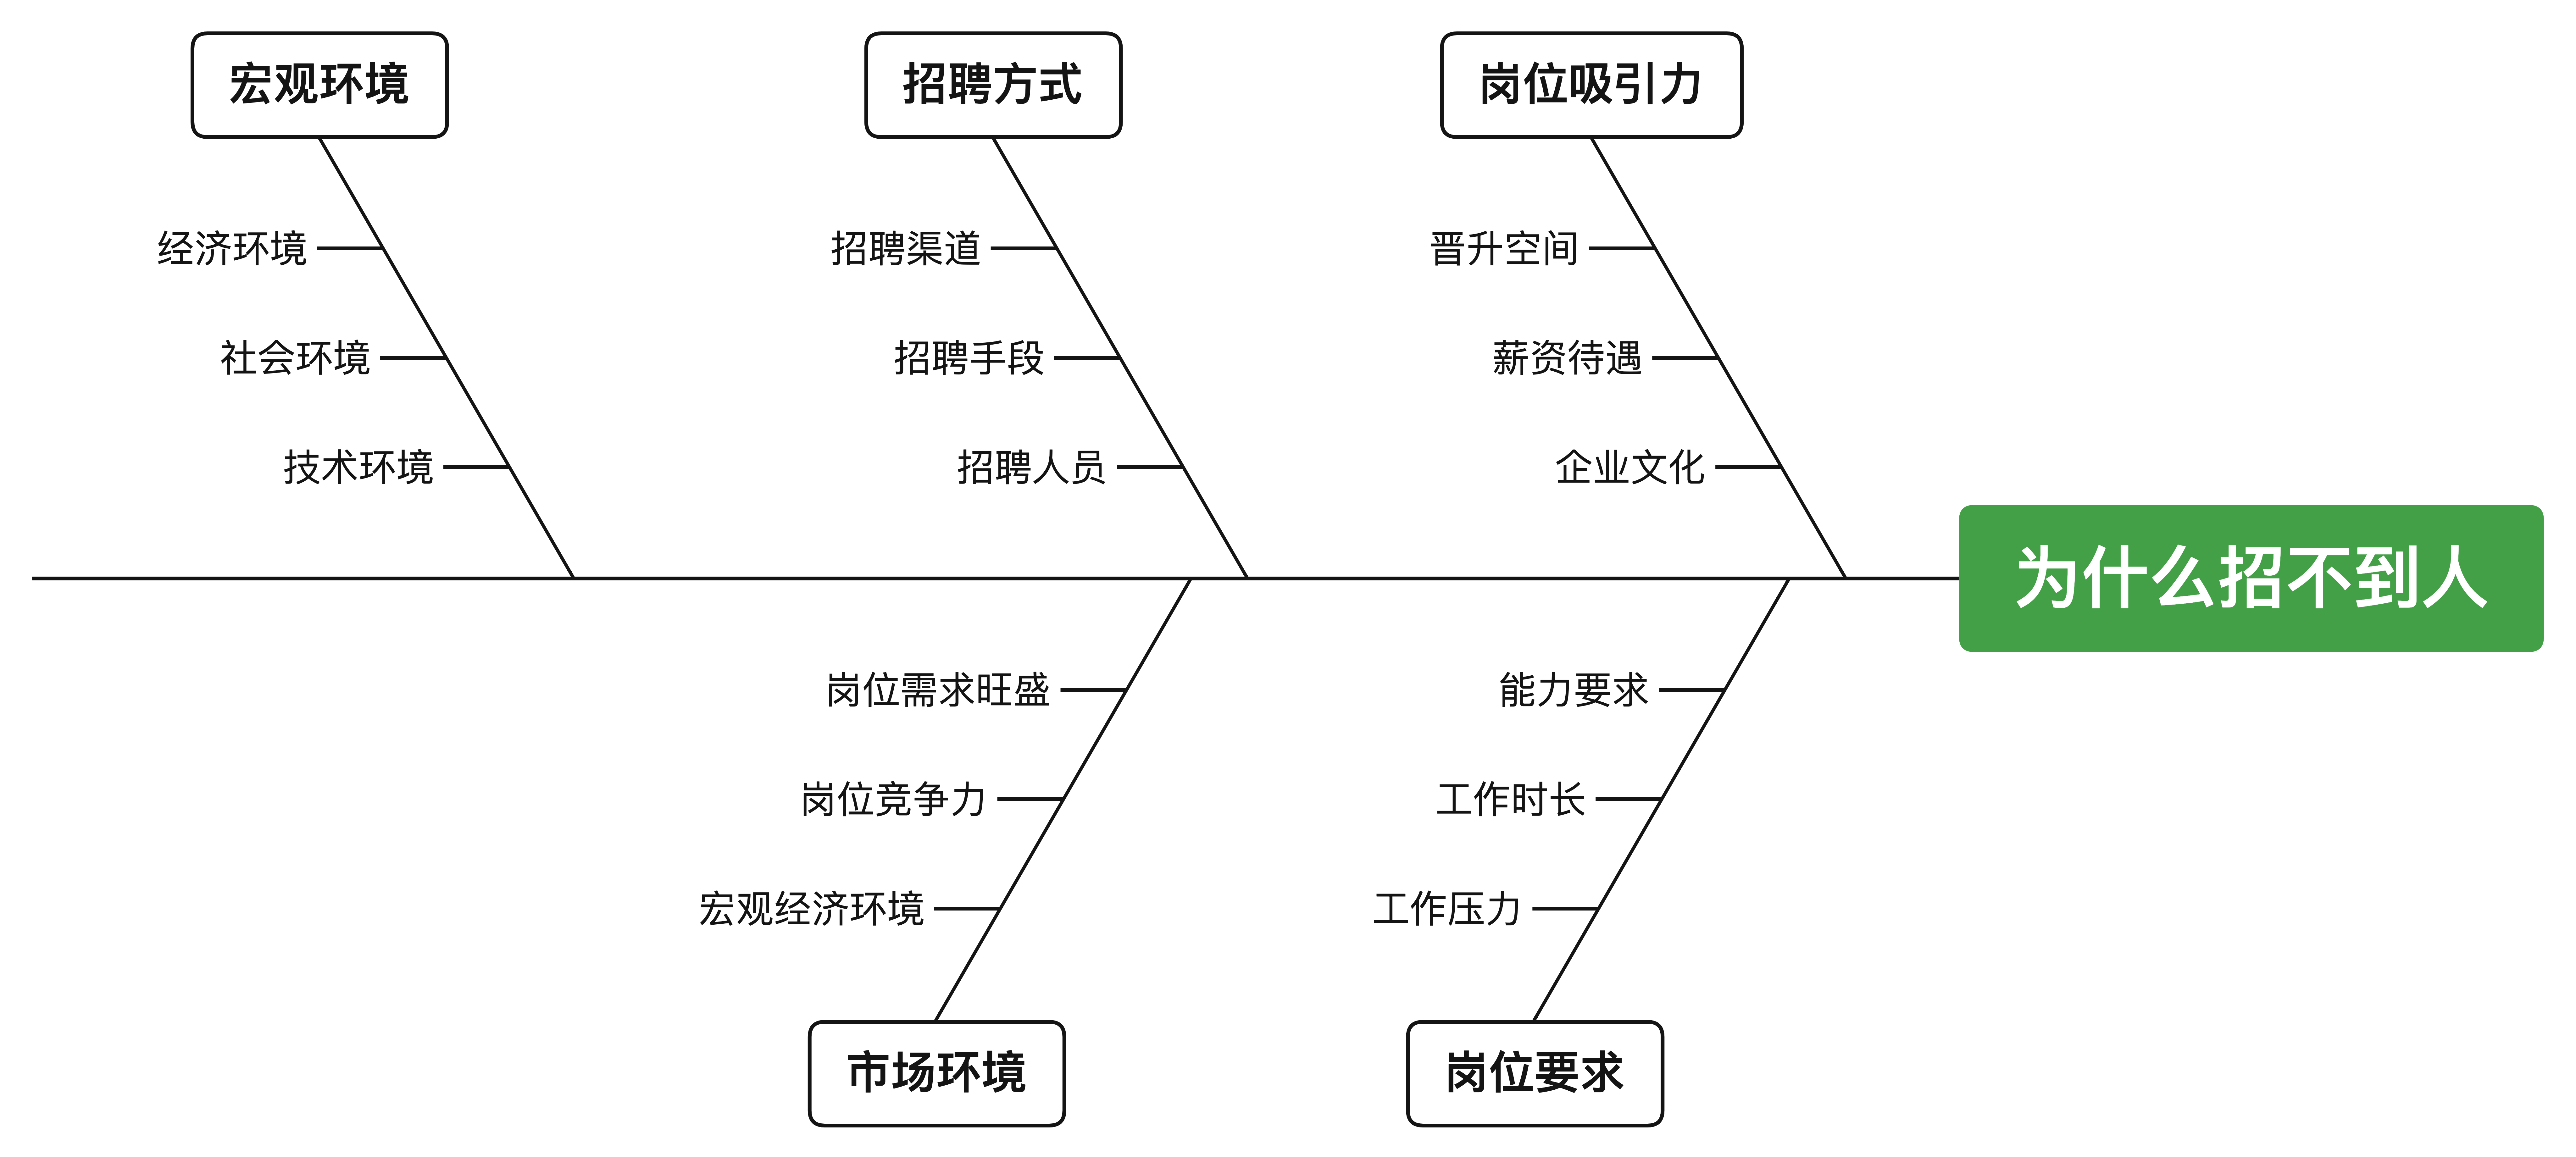
\includegraphics[width=0.50\textwidth]{鱼骨分析法_5.png}
  \end{center}
\end{figure}
%
或者在思考产品满意度下降时也可以用鱼骨分析法来探究问题产生的原因。
%
\begin{figure}[H]
  \begin{center}
    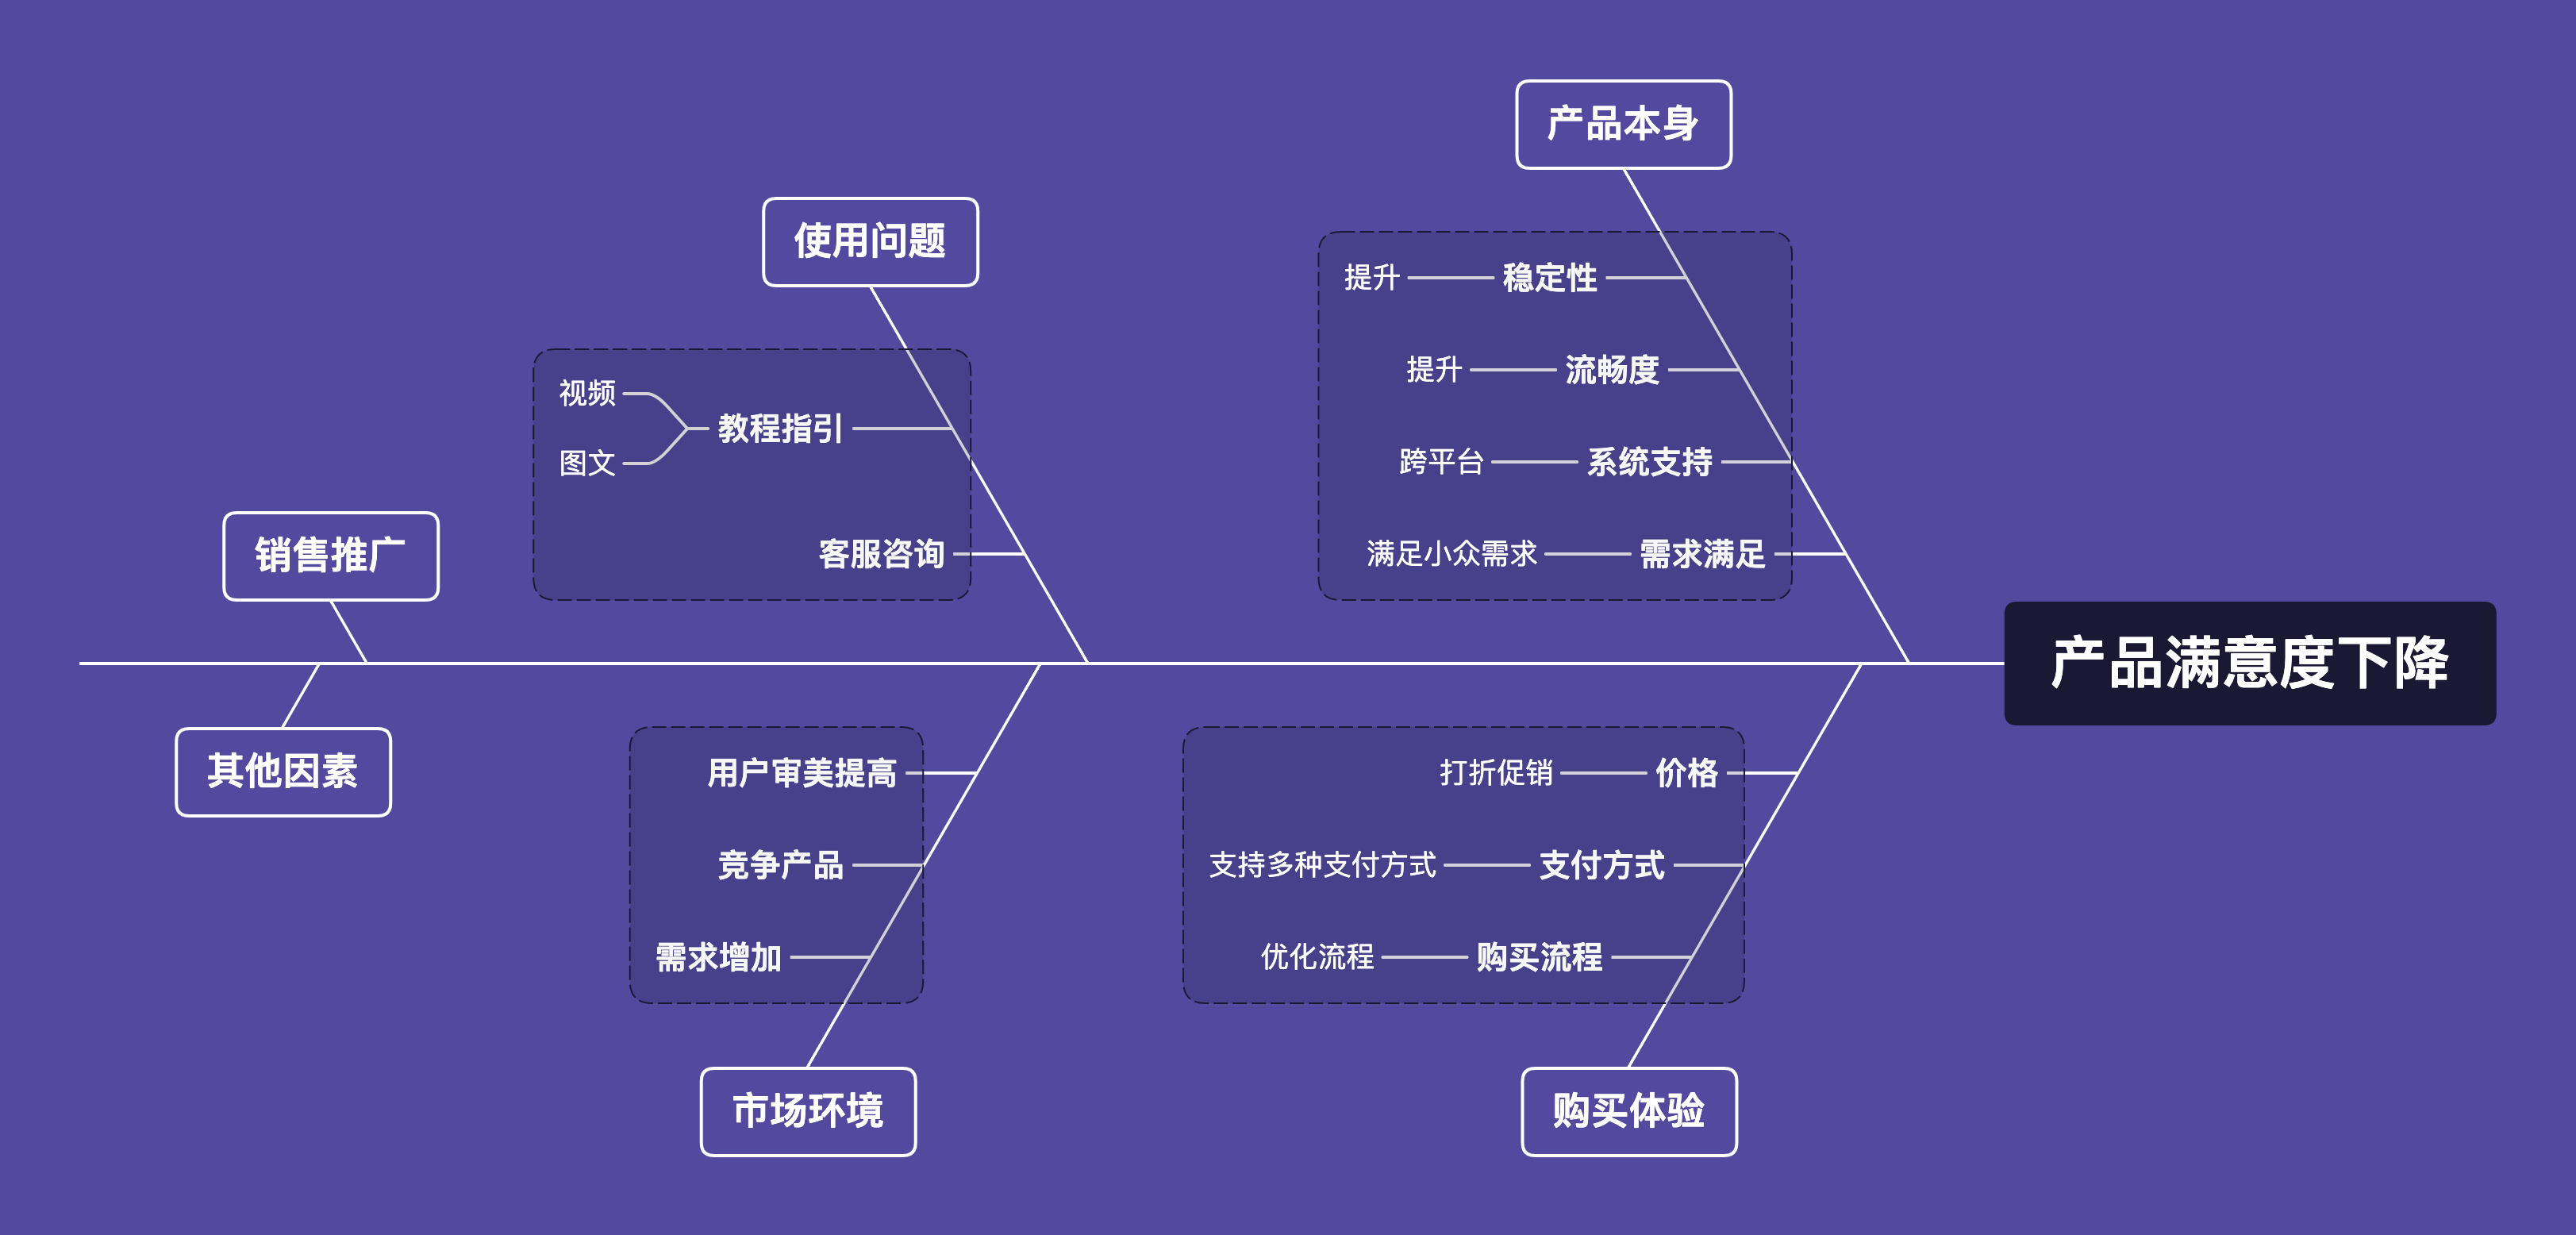
\includegraphics[width=0.50\textwidth]{鱼骨分析法_6.png}
  \end{center}
\end{figure}
%
\subsection{对策分析}
有问题即有对策。面临难题时,找出原因很重要,
根据原因找到相应的对策也很重要。在进行对策分析时,
用鱼骨分析法也是一个很好的思路。
比如下图针对提高设备效率的应对措施鱼骨图。
%
\begin{figure}[H]
  \begin{center}
    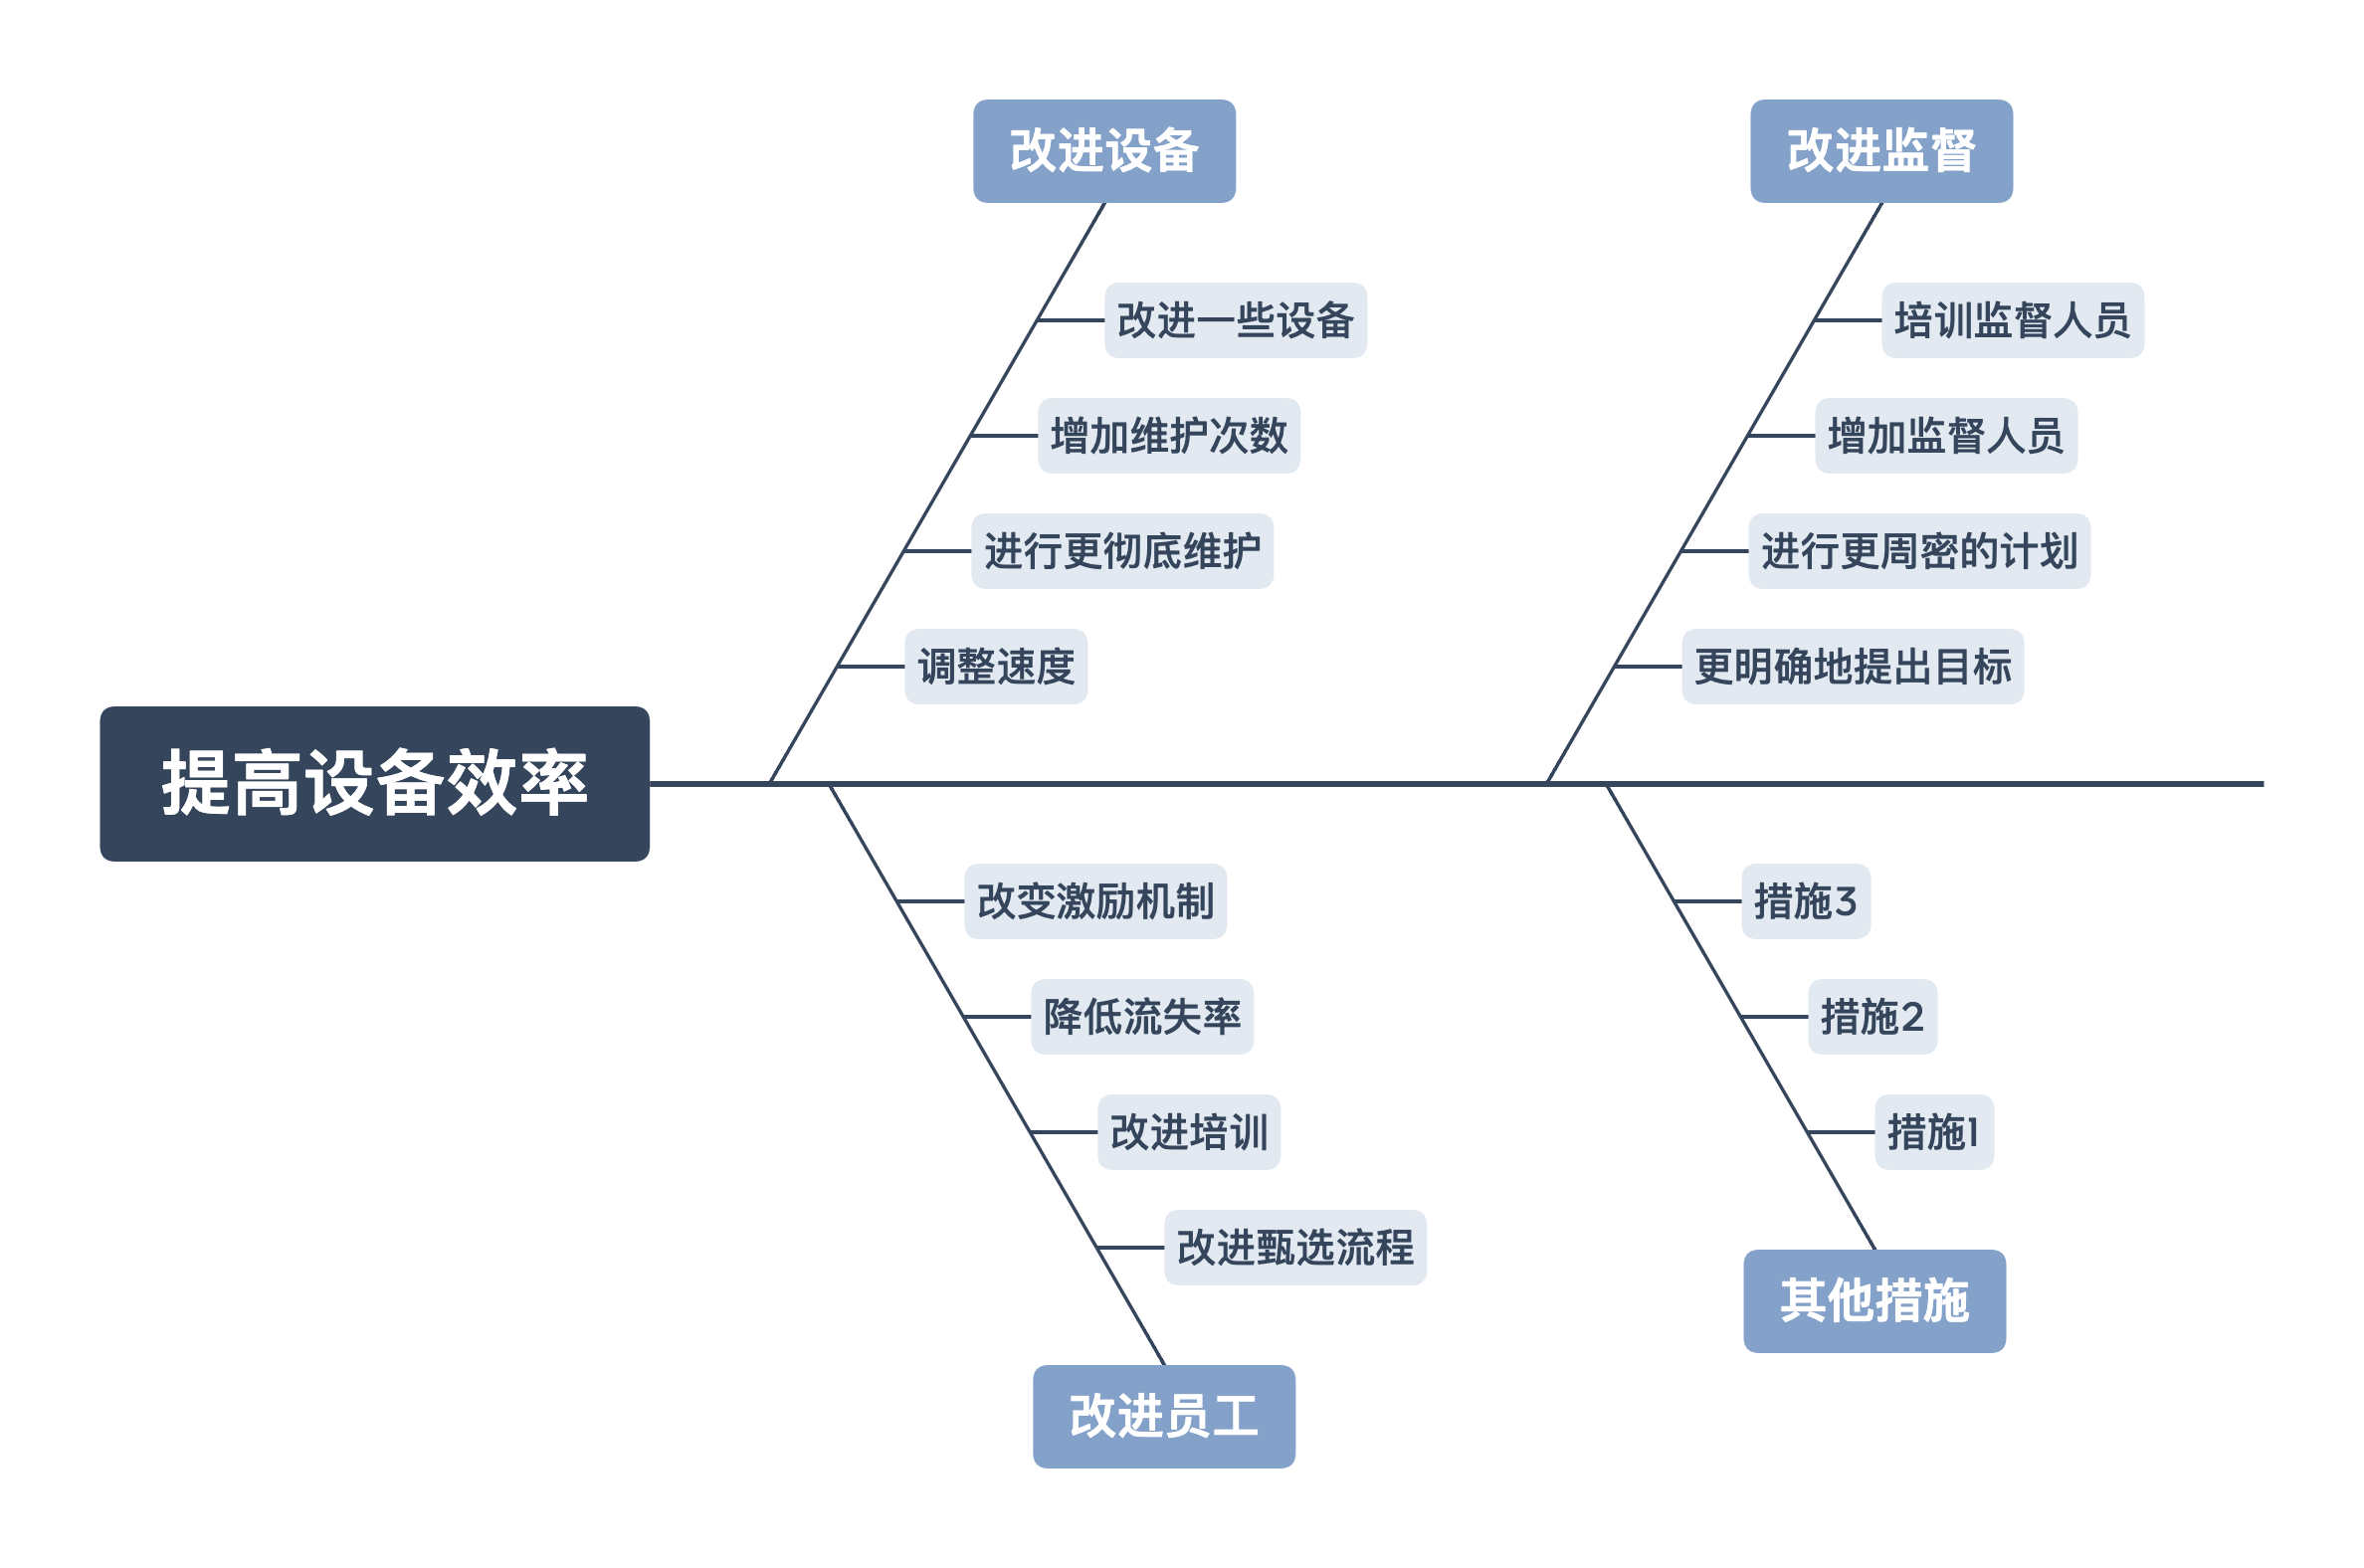
\includegraphics[width=0.50\textwidth]{鱼骨分析法_7.png}
  \end{center}
\end{figure}
%
还有以下面对拖延顽疾时相应的对策分析图。当你对现状产生不满,
对自身所处的境遇不满时,不妨找个安静的时刻,认真审视和反思下自己想改变的地方,
找出原因,想好对策。
%
\begin{figure}[H]
  \begin{center}
    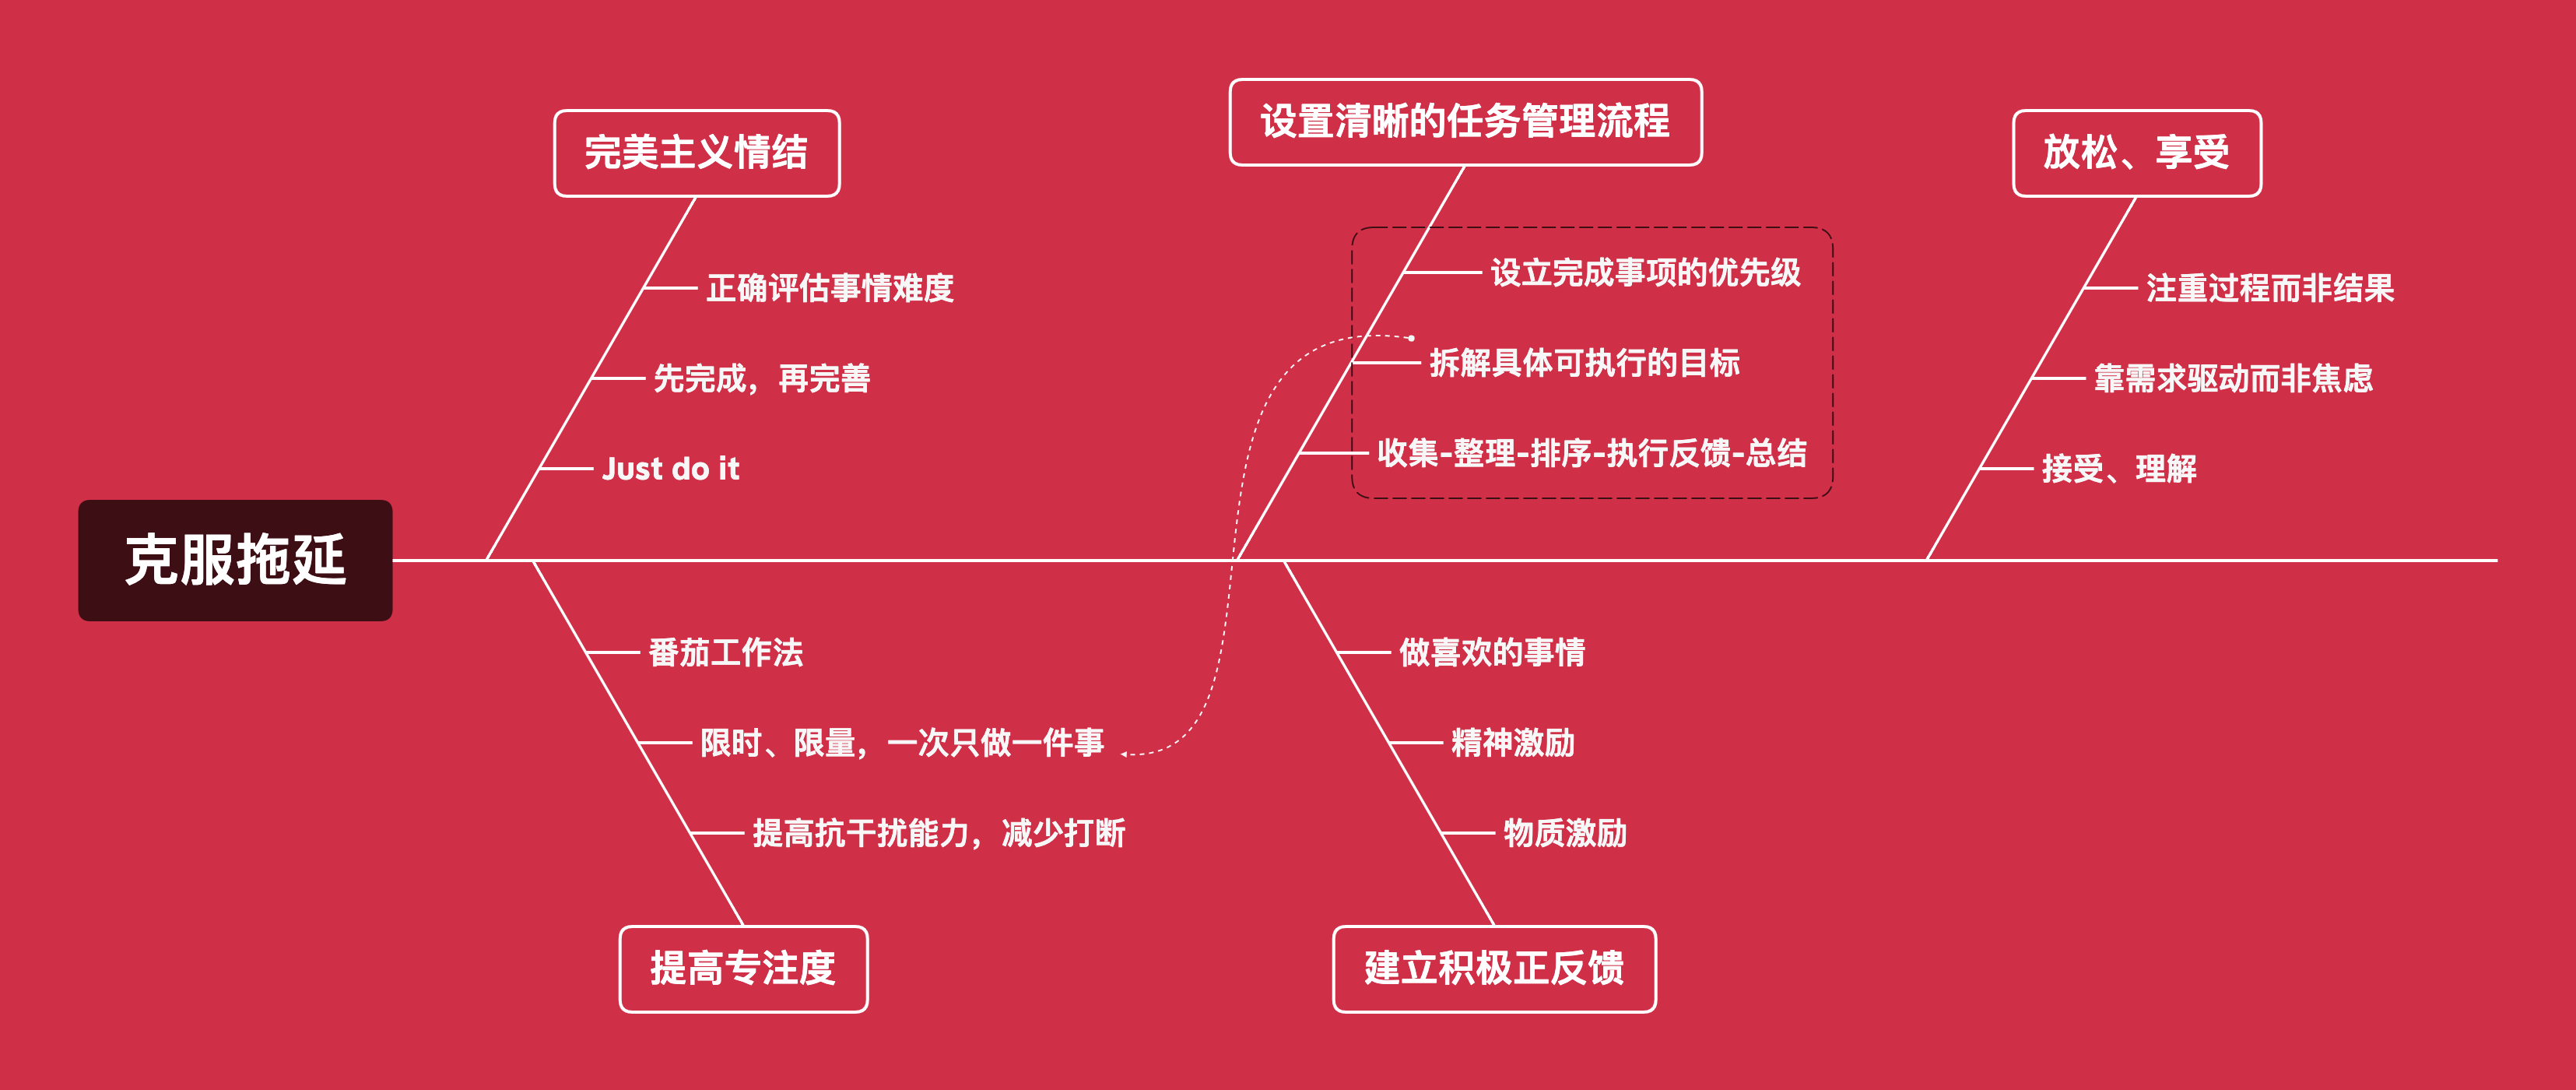
\includegraphics[width=0.50\textwidth]{鱼骨分析法_8.png}
  \end{center}
\end{figure}
%
绘制鱼骨图并不难,难的是层层深入,不断向下深挖各种原因。
%
\end{document}
